\documentclass[12pt]{article} \setlength{\oddsidemargin}{0in}
\setlength{\evensidemargin}{0in} \setlength{\textwidth}{6.5in}
\setlength{\parindent}{0in} \setlength{\textwidth}{16cm}
\setlength{\topmargin}{1in} \addtolength{\topmargin}{-1.5in}
\setlength{\textheight}{23cm} \setlength{\parskip}{0.75cm}

% Brackets
\usepackage{mathtools, tikz-qtree} \DeclarePairedDelimiter\ceil{\lceil}{\rceil}
\DeclarePairedDelimiter\floor{\lfloor}{\rfloor}

% Tikz settings
\usepackage{tikz} \usetikzlibrary{trees} \usetikzlibrary {positioning}
\definecolor {mypurple}{cmyk}{0.6,0.4,0.1,0} \definecolor
{myred}{cmyk}{0,0.3,0.3,0} \usetikzlibrary{fit,shapes.misc}

% Typesetting options
\usepackage{fancyvrb} \usepackage{amsmath,amsfonts,amssymb, mathdots}
\usepackage [english]{babel} \usepackage [autostyle, english =
american]{csquotes} \usepackage[none]{hyphenat} \usepackage{url}


% Graph
\usepackage{tikz}
\tikzstyle{level 7} = [level distance = 1.5cm , sibling distance = .5cm]
\tikzstyle{level 6} = [level distance = 1cm , sibling distance = .5cm]
\tikzstyle{level 5} = [level distance = 1cm , sibling distance = .5cm]
\tikzstyle{level 4} = [level distance = 1cm , sibling distance = .5cm]
\tikzstyle{level 3} = [level distance = 1cm , sibling distance = .5cm]
\tikzstyle{level 2} = [level distance = 1cm , sibling distance = .5cm]
\tikzstyle{level 1} = [level distance = 1cm , sibling distance = .5cm]

\usepackage{graphicx}
\graphicspath{ {images/} }
\graphicspath{ {\string~/Desktop/} }

\usepackage {fancyvrb}
\newenvironment{qv}
{\quote\Verbatim}{\endVerbatim\endquote}

\usetikzlibrary{trees}
\tikzset{every tree node/.style={minimum width=2em,draw,rectangle, top color=white, bottom color=blue!40},
         blank/.style={draw=none},
         edge from parent/.style=
         {draw,edge from parent path={(\tikzparentnode) -- (\tikzchildnode)}},
         level distance=1.5cm}

\begin{document}

\noindent CSCI 3104 Spring 2018 \hfill Problem Set 5\\
Erika Bailon (09/28)

\hrulefill

{\fontfamily{cmr}\selectfont

  % ******************* PROBLEM 1 *********************
  \section*{Problem 1}

  \textit{(15 pts) Bellatrix Lestrange is writing a secret message to Voldemort and wants to
prevent it from being understood by meddlesome young wizards and Muggles. She
decides to use Huffman encoding to encode the message. Magically, the symbol frequencies of the message are given by the Pell numbers, a famous sequence of integers
known since antiquity and related to the Fibonacci numbers. The \textbf{n}th Pell number is
defined as $P_n = 2 P_{n_1} + P_{n-2}$ for $n > 1$ with base cases $P_0 = 0$ and $P_1 = 1$.}

  \begin{enumerate}
  \item[(a)]{\textit{For an alphabet of $ \Sigma = \{a, b, c, d, e, f, g, h\}$ with frequencies given by the first $|\Sigma|$ non-zero Pell numbers, give an optimal Huffman code and the corresponding
encoding tree for Bellatrix to use.}}
    \\
    Given the conditions $P_n = 2 P_{n_1} + P_{n-2}$ ; $P_0 = 0$ , $P_1=1$ , and the first Pell number is non-zero, then we obtain:\\\\
    $P_1(a) = 1\\
    P_2(b) = 2(1) + 0 = 2\\
    P_3(c) = 2(2) + 1 = 5\\
    P_4(d) = 2(5) + 2 = 12\\
    P_5(e) = 2(12) + 5 = 29\\
    P_6(f) = 2(29) + 12 = 70\\
    P_7(g)= 2(70) + 29 = 169\\
    P_8(h) = 2(169) + 70 = 408$
    \begin{align*}
		a &= 1
        &
        b &= 2
        &
        c &= 5
        &
        d &= 12\\
        e &= 29
        &
        f &= 70
        &
        g &= 169
        &
        h &= 408\\
	\end{align*}
    The Huffman code:\\
    $a = 0000000\\
    b=0000001\\
    c=000001\\
    d=00001\\
    e=0001\\
    f=001\\
    g=01\\
    h=1$\\\\
    The encoding tree looks like this:\\ 
\begin{tikzpicture}{c}
  \Tree
  [. {$ 696$}
  	[.{$ 288 $}
		[.119
			[.{$49$}
			[.{$20$}
			[.{$8$}
			[.{$3$}
			[.{$a$}
			]
			[.{$b$}
			]
			]
			[.{$c$}
			]
			]
			[.{$d$}
			]
			]
			[.{$e$}
			]
			]
			[.{$f$}
			]
		]
		[.{$g$}
		]
    	]
  	[.{$ h$}
    ]
  ]
  \end{tikzpicture}
    	
    
  \item[(b)]{\textit{Generalize your answer to (1a) and give the structure of an optimal code when
the frequencies are the first n non-zero Pell numbers.}}
    \\\\
     %******************** b *********************%
    For the general case, we take in consideration that the frequencies are the first non-zero Pell numbers. Therefore, we get that:\\\\
    $P_n = 1\\
    P_{n-1} = 01\\
    P_{n-2} = 001\\
    P_{n-3} = 0001\\
    \cdot\\
    \cdot\\
    \cdot\\
    P_{n-k} = 0^{n-k}1\\
    P_3 = 0^{n-3}1\\
    P_2 = 0^{n-2}1\\
    P_1 = 0^{n-1} $\\\\\\
    (Tree next page)\\
    \begin{tikzpicture}{c}
  \Tree
  [. {$\sharp$}
  	[.{$ \sharp $}
		[.{$\sharp$}
			[.{$\iddots$}
			[.{$\sharp$}
			[.{$\sharp$}
			[.{$\sharp$}
			[.{$P_1$}
			]
			[.{$P_2$}
			]
			]
			[.{$P_3$}
			]
			]
			[.{$P_4$}
			]
			]
			[.{$\cdot \cdot \cdot$}
			]
			]
			[.{$P_{n-2}$}
			]
		]
		[.{$P_{n-1}$}
		]
    	]
  	[.{$P_n$}
    	]
  ]
  \end{tikzpicture}
  \end{enumerate}

  \newpage

  % ******************* PROBLEM 2 *********************
  \section*{Problem 2}

  \textit{(30 pts) A good hash function $h(x)$ behaves in practice very close to the uniform hashing
assumption analyzed in class, but is a deterministic function. That is, $h(x) = k$ each
time $x$ is used as an argument to $h(x)$. Designing good hash functions is hard, and a
bad hash function can cause a hash table to quickly exit the sparse loading regime by
overloading some buckets and under loading others. Good hash functions often rely
on beautiful and complicated insights from number theory, and have deep connections
to pseudorandom number generators and cryptographic functions. In practice, most
hash functions are moderate to poor approximations of uniform hashing.}

\textit{Consider the following hash function. Let $U$ be the universe of strings composed of the
characters from the alphabet $\Sigma = [A, \dots ,Z]$, and let the function $f(x_i)$ return the index
of a letter $x_i \in \Sigma$, e.g., $f(A)=1$ and $f(Z)=26$. Finally, for an \textbf{m}-character string
$x \in \Sigma^m$, define $h(x)=([\sum_{i=1}^m f(x_i)] \ \text{mod} \ l)$, where $l$ is the number of buckets in the hash table. That is, our hash function sums up the index values of the characters of a
string $x$ and maps that value onto one of the $l$ buckets.}

\begin{enumerate}
\item[(a)]
  %******************** a *********************%
  Here is the output of my hashing. We can see a bell shape because of the strings we were inputting. Most last names' length is about the same, that is why is not uniform.  
  \begin{figure}[h]
\includegraphics[width=13cm,height = 10cm]{2a}
\end{figure}

And here is the code (including part c): \\
 \begin{qv}
#Erika Bailon 09/28
#Algorithms

import sys
import random
import math
import numpy as np
import matplotlib.mlab as mlab
import matplotlib.pyplot as plt

#can read any file and we have set always the buckets' #
l=200
filename = sys.argv[1]

randomlySelectedNames=[]
newArr=[]
newArr2=[]
collisions=[]

# get 50% random names from input file
with open(filename) as f:
	for line in f:
		newArr.append(line)

for i in newArr:
	i = i.split(" ",1)	#get the elements from the first column
	newArr2.append(i[0])

namesSize=len(newArr2)
halfSize=namesSize//2

#randomize using their original index - later the index will be 
#reset with the randomized last names
for i in range(0,halfSize):
	index=random.choice(newArr2)
	randomlySelectedNames.append(index)
	newArr2.remove(index)

# make array to count collisions
for i in range(0,200):
	collisions.append(0)

# fake the hash
hashFake=[]
for name in randomlySelectedNames:
	f=0
	for i in range(0,len(name)):
		f=f + (ord(name[i])-ord('A')+1)
		f=f%l;
	hashFake.append(f)
	# increment colisions
	collisions[f] += 1

#find largest hashed amount
largest = 0
for i in range(0,len(collisions)):
	if (collisions[i] > largest):
		largest = collisions[i]

print(collisions)

#lets print the histogram!
num_bins = 200
n, bins, patches = plt.hist(hashFake, num_bins, facecolor='blue', alpha=0.5)
plt.xlabel('hash location')
plt.ylabel('# of times hashed at this location')
plt.show()

#info for the plot 
name_index = []
name_index.extend(range(1,44400))
hash_uniform = []
rb_tree = []
theta = []

for i in name_index:
	if((i/halfSize) < 1):
		hash_uniform.append(0)
	else:
		hash_uniform.append(i/halfSize)
	rb_tree.append(2*np.log(i+1))
	theta.append(i/75)

#failed try to print a perfect plot =( almost perfect tho
plt.plot(name_index,hashFake)
plt.plot(name_index,hash_uniform,linewidth=4)
plt.plot(name_index,rb_tree,linewidth=4)
plt.plot(name_index,theta,linewidth=4)
plt.title('Hash entries and longest chain')
plt.ylabel('Longest Chain')
plt.xlabel('Hash Table')
plt.show()

  \end{qv}
  
 And here is the array that contains the collisions, different from the array that contains all the math operations though. \\
 $[0, 0, 0, 0, 0, 0, 1, 4, 4, 2, 7, 0, 6, 7, 8, 7, 18, 13, 19, 21, 25, 33, 33, 39, 50, 53, 53, 81, 78, 84,\\ 
 116, 106, 120, 146, 165, 153, 194, 181, 201, 206, 269, 283, 315, 290, 309, 348, 403, 389, 381,\\
  427, 430, 452, 458, 501, 537, 551, 560, 610, 590, 616, 595, 701, 662, 671, 727, 720, 667, 705,\\
   729, 718, 697, 744, 689, 750, 756, 728, 699, 668, 686, 716, 734, 673, 650, 675, 671, 622,\\
    676, 604, 594, 610, 607, 569, 561, 509, 463, 482, 461, 426, 417, 421, 375, 374, 371, 317, \\
    325, 330, 348, 277, 273, 296, 263, 235, 235, 232, 211, 172, 199, 167, 176, 166, 155, 160, \\
    145, 125, 148, 123, 122, 110, 112, 94, 98, 93, 77, 73, 65, 70, 66, 55, 58, 40, 51, 42, 37, 34,\\
     45, 29, 29, 30, 36, 27, 23, 25, 17, 19, 12, 15, 17, 10, 17, 16, 16, 11, 8, 11, 7, 9, 4, 6, 4, 3, 4, \\
     7, 5, 2, 4, 3, 2, 4, 3, 1, 2, 1, 1, 5, 0, 2, 0, 1, 0, 0, 1, 1, 0, 0, 0, 1, 0, 1, 1, 0]$


\item[(b)]{\textit{Enumerate at least 4 reasons why $h(x)$ is a bad hash function relative to the ideal behavior of uniform hashing.}}
  \\\\
   %******************** b*********************%
   $1.$ A good hashing function is deterministic, this means that we should obtain always the same hash values with the file input. Our function h(x) does not have this property since we are generating random values each time we pass the file to our program. \\
   $2.$ A good hashing function is uniform, this means that all the data is expected to have an even distribution, in the input and output. The function $h(x)$  does not have uniformity since the stings we are using as input have a diverse range of value and do not map any evenly output. This is, most of the names fall into the same category of length, this produces and uneven output.  \\
   $3.$ Another reason is that the alphabet is not being using uniformly either. Some letters like the vocals, are used many more times than other letters, like $z$.\\
   $4.$ A good hashing function uses all of the data in the file in order to create a good hash table. In our function $h(x)$ we are only taking randomly $50\%$ of our file, which does not provide a good hash table from the input file. \\
   $5.$ A good hash function can use the same string as input and still generated different value on the output. Out function $h(x)$ will generate the same output value if we pass the same strings because we have a set number for the value of each letter int he string based in the alphabet, therefore the same string will output the same value. \\
   $6.$ Our bad hash function has a large number of a bucket. If we were to use a bucket number = $26$, we would have a better distribution since we have 26 letters in the alphabet. The fact that we are making our number of buckets bigger, is what it creates a bell shape on out output. \\
\item[(c)]{\textit{Produce a plot showing (i) the length of the longest chain (were we to use chaining for resolving collisions) as a function of the number $n$ of these strings that we hash
into a table with $l = 200$ buckets, and (ii) the exact upper bound on the depth
of a red-black tree with $n$ items stored.}

\textit{Then, (i) comment on the value of $n$ at which the red-black tree becomes a more
efficient data structure, and (ii) state the length of the longest chain when every
bucket has at least one hash hit.}}
  \\\\
   %******************** c *********************%
   This is the output I get for my plot. \\
    \begin{figure}[h]
\includegraphics[width=13cm,height = 10cm]{2c}
\end{figure}


\end{enumerate}

\newpage

% ******************* PROBLEM 3 *********************
\section*{Problem 3}
\textit{Draco Malfoy is struggling with the problem of making change for $n$ cents
using the smallest number of coins. Malfoy has coin values of $v_1 < v_2 < \dots < v_r $ for r
coins types, where each coin�?s value $v_i$ is a positive integer. His goal is to obtain a set
of counts $\{ d_i \}$, one for each coin type, such that $\sum_{i=1}^r d_i=k$ and where $k$ is minimized.}
\begin{enumerate}
\item[(a)]{\textit{A greedy algorithm for making change is the \textbf{cashier�?s algorithm}, which all young wizards learn. Malfoy writes the following pseudocode on the whiteboard
to illustrate it, where $n$ is the amount of money to make change for and v is a
vector of the coin denominations:}
}
\begin{verbatim}
wizardChange(n,v,r) :
  d[1 .. r] = 0
  // initial histogram of coin types in solution
  while n > 0 {
    k = 1
    while ( k < r and v[k] > n ) { k++ }
    if k==r { return �?no solution�? }
    else { n = n - v[k] }
  }
  return d
\end{verbatim}

\textit{Hermione snorts and says Malfoy�?s code has bugs. Identify the bugs and explain
why each would cause the algorithm to fail. }
  
   %******************** a *********************%
   (last brackets of the code and explanation continues in next page)
   
    \begin{qv}
    wizardChange(n,v,r):
    d[1...r] = 0
    while n > 0 {
        k = r                              *
        while ( k > 0 and v[k] > n )       **
        {
            k--                            ***
        }
        if k == 0                          ****
        {
            return 'no solution'
        }
        else
        {
            d[k] += 1                      *****
            n = n-v[k]
        }
    }
    \end{qv}
    Changes:\\
    * The first change that needed to be made was to set $k=r$ because it needs to start at the greatest element to be a greedy algorithm. \\
    **The second, changed to $k>0$ because of the previous change, we need to make sure the loop is the right range.\\
    *** The third change was to decrement $k--$ because we are starting at the last element so we need to go back in the array. \\
    ****Fourth, changed because our $k$ already equals $r$ so since we are going back now we have to exit when $k==0$.\\
    ***** Last change, we need to increment $d$ because we cannot return it as it was in the beginning. So now $d[k] += 1 $ will output the number of times the denomination is used. \\

  
\item[(b)]{\textit{Sometimes the goblins at Gringotts Wizarding Bank run out of coins\footnote{It�?s a little known secret, but goblins like to eat the coins. It isn�?t pretty for the coins, in the end.} and make change using whatever is left on hand. Identify a set of U.S. coin denominations
for which the greedy algorithm does not yield an optimal solution. Justify your
answer in terms of optimal substructure and the greedy-choice property. (The set
should include a penny so that there is a solution for every value of $n$.)}}
  \\\\
   %******************** b *********************%
Lets assume that our U.S. coin denomination are .01, .05 and .25, where we are missing the dime coin. Now assume we need to give change for  1.70. \\
Under our greedy algorithm the distribution should look like this:
\begin{verbatim}
Quarters: 6 
Dimes: 2 
Nickels: 0 
Pennies: 0 
Total coins used: 8 
\end{verbatim}
Given the condition of missing a coin, in this case a dime, the distribution would look like this: 
\begin{verbatim}
Quarters: 6 
Nickels: 4 
Pennies: 0 
Total coins used: 10 
\end{verbatim}

For an input of U.S. currency wanting a maximum greedy return of coin distribution we will run into a problem if one of the coins is missing. Our greedy algorithm looks for the coin with a value less than the output needed. If one of our coins is missing, then the algorithm will move on to the next smallest denomination. When this happens we will always end up giving back more coins than is optimal because of the missing coin.  \\

\item[(c)]{\textit{(8 pts extra credit) On the advice of computer scientists, Gringotts has announced that they will be changing all wizard coin denominations into a new set of coins
denominated in powers of $c$, i.e., denominations of $c_0$, $c_1$, $\dots$, $c^l$ for some integers
$c > 1$ and $l \ge 1$. (This will be done by a spell that will magically transmute old
coins into new coins, before your very eyes.) Prove that the cashiers algorithm
will always yield an optimal solution in this case.}

\footnotesize{\textit{Hint: first consider the special case of $c = 2$.}}}
  \\\\
  Let's consider the case when our $c$ has a value of $2$. Our coin denomination would be \(c^0,c^1,c^2...c^l\) which will be:\\
  smallest coin = 1\\
  next biggest coin = 2\\
  next = 4\\
  next = 8...\\
  until we have $2^l$\\
  Let's first look at the case of c=2. \\
IF we use the cashiers algorithm we would start at the biggest denomination  and find the optimal distribution of coins.\\
Now, if we have an input where $c = k$ and $k>=2$, we can use induction to prove that the algorithm will work. \\
Assume we have $c = k+1$. We are going to raise $k+1$ to the power of \textit{l}. \\
$(k+1)^0 = 1$ \\
 $(k+1)^0 \leq (k+1)^1$ \\
 $(k+1)^1 \leq (k+1)^2$\\
$ \cdot $\\
$ \cdot $\\
$ \cdot $\\
 $(k+1)^{l-1} \leq (k+1)^l$ \\
Our last element is greater than any other element in the array. Therefore, for any input k our cashier's algorithm will always choose the optimal solution. \\\\\\\\
WORKED WITH:::\\
Selena Quintanilla, Eric OropezaElwood, Jason Lubrano, CAs, and office hours. 
\end{enumerate}
% ---------------------------------------------------
\end{document}









